% ============================================================================
% IEEE conference-format project report
% Single-Cycle 32-bit MIPS Processor with Memory Interface
% Build:  cd report && tectonic main.tex     (or: pdflatex main && bibtex main && pdflatex main x2)
% ============================================================================
\documentclass[conference]{IEEEtran}
\IEEEoverridecommandlockouts

\usepackage{cite}
\usepackage{amsmath,amssymb}
\usepackage{graphicx}
\usepackage{booktabs}
\usepackage{multirow}
\usepackage{array}
\usepackage{xcolor}
\usepackage{listings}
\usepackage[section]{placeins}
\usepackage[hidelinks]{hyperref}

\graphicspath{{../docs/diagrams/}{../docs/waveforms/}}

% ---- results that come from the synthesis run -------------------------------
% Results from synthesis/run_yosys.sh (nextpnr-himbaechel, GW5AST-138, post-placement STA)
\newcommand{\fmaxvalue}{30.46~MHz}
\newcommand{\gowinrows}{%
LUT4 & 25{,}695 & 138{,}240 & 18.6\% \\
MUX2 (wide muxes) & 11{,}488 & 138{,}240 & 8.3\% \\
DFF & 8{,}446 & 138{,}240 & 6.1\% \\
ALU (carry) & 106 & 103{,}680 & 0.1\% \\
BSRAM & 1 & 340 & 0.3\% \\
IOB & 8 & 324 & 2.5\% \\}


\lstset{basicstyle=\ttfamily\scriptsize, columns=fullflexible, frame=single,
        breaklines=true, xleftmargin=2pt, xrightmargin=2pt}

\begin{document}
\sloppy
\setlength{\emergencystretch}{2em}

\title{Design, Verification and FPGA Synthesis of a\\
32-bit Single-Cycle MIPS Processor with Memory Interface\\[4pt]
\large Modern Computer Architecture -- Project 2, B.Tech (CS\&AI)}

\author{
\IEEEauthorblockN{Gauri Jindal, Sanchit Garg, Manas Saxena, Tanish Garg}
\IEEEauthorblockA{\textit{Newton School of Technology, Rishihood University}, India}
}

\maketitle

% ============================================================================
\begin{abstract}
This report presents the design, verification and FPGA synthesis of a 32-bit
single-cycle processor that implements a subset of the MIPS32 instruction set
architecture in synthesizable Verilog-2001. The processor executes R-type
arithmetic and logic instructions (\texttt{add}, \texttt{sub}, \texttt{and},
\texttt{or}, \texttt{slt}), memory instructions (\texttt{lw}, \texttt{sw}),
\texttt{addi}, the conditional branch \texttt{beq} and the unconditional jump
\texttt{j}, each in exactly one clock cycle. The design is partitioned into
ten modules: program counter, instruction memory, main control unit, ALU
control, register file, sign extension, ALU, data memory, branch/jump logic and
the top-level integration. A Harvard-style memory interface provides a
$256\times32$ instruction ROM and a $256\times32$ data RAM with address
validation. Every module has a self-checking testbench, and the integrated CPU
executes four machine-code programs (array sum, maximum search, factorial and a
jump/logic test); all 129 directed checks pass in Icarus Verilog. Measured
dynamic instruction counts give a CPI of 1.00 against 3.71 for an equivalent
multi-cycle design. Synthesis for a Xilinx Artix-7 device uses 4{,}190 LUTs and
9{,}216 flip-flops, and place-and-route with static timing analysis on a Gowin GW5AST
FPGA gives a maximum operating frequency of \fmaxvalue.
\end{abstract}

\begin{IEEEkeywords}
MIPS, single-cycle processor, datapath, control unit, Verilog HDL,
memory interface, FPGA synthesis, CPI
\end{IEEEkeywords}

% ============================================================================
\section{Introduction}
A processor is the combination of a \emph{datapath}, which stores and
transforms data, and a \emph{control unit}, which decodes each instruction and
steers the datapath~\cite{patterson2014cod}. The single-cycle organization is
the simplest correct implementation of an instruction set: every instruction
is fetched, decoded, executed, and its result written back within one clock
period. It is the reference point from which multi-cycle and pipelined
designs are derived and compared~\cite{hennessy2019caqa}.

The objective of this project (Project~2 of the Modern Computer Architecture
course) is to implement a 32-bit single-cycle MIPS processor that executes
arithmetic, memory and branch instructions, to load and run small programs
such as an array sum, a maximum search and a factorial, and to verify,
synthesize and analyse the design. The specific contributions are:
\begin{itemize}
  \item a modular, synthesizable Verilog-2001 RTL implementation of the
        datapath, control unit and Harvard memory interface;
  \item self-checking testbenches for every module and for the full CPU, with
        waveform evidence of instruction execution;
  \item a quantitative performance study (instruction mix, cycles, CPI and
        execution time) against a multi-cycle baseline; and
  \item FPGA synthesis and place-and-route results, including resource
        utilization and maximum operating frequency.
\end{itemize}

% ============================================================================
\section{Literature Review}

\subsection{RISC and the MIPS architecture}
Patterson and Ditzel argued that a reduced instruction set with simple,
fixed-length instructions allows a simpler and faster implementation than the
complex instruction sets of the time~\cite{patterson1980risc}. The Stanford MIPS
project put this into practice with a load/store architecture, a large general
purpose register file and instruction formats designed for single-cycle
decoding~\cite{hennessy1982mips}. The commercial MIPS architecture that followed
defines three instruction formats (R, I and J), 32 general-purpose registers
with \texttt{\$zero} hard-wired to zero, and byte-addressed, word-aligned
memory accesses~\cite{kane1992mips,mips32vol2}. These properties make MIPS the
standard teaching ISA for processor design: the opcode in bits $[31{:}26]$
selects the format, and register specifiers are always in the same bit
positions, so register reads can begin before decoding is complete.

\subsection{Single-cycle, multi-cycle and pipelined organizations}
Patterson and Hennessy derive the single-cycle MIPS datapath from the
requirements of each instruction class and add multiplexers (RegDst, ALUSrc,
MemtoReg, PCSrc) that are driven by a combinational main decoder and a
two-level ALU decoder~\cite{patterson2014cod}. Harris and Harris present the
same microarchitecture directly in HDL and use it as the starting point for
multi-cycle and pipelined versions~\cite{harris2013ddca}. The single-cycle
design has CPI~$=1$, but its clock period is set by the slowest instruction
(\texttt{lw}), which passes through instruction memory, register file, ALU,
data memory and register write. Multi-cycle designs divide execution into
shorter steps (CPI between 3 and 5 for MIPS) so that simple instructions finish
earlier, and pipelined designs overlap these steps to approach CPI~$=1$ at a
short clock period~\cite{hennessy2019caqa}. The single-cycle CPU is therefore
the correct baseline for later pipelining and hazard studies.

\subsection{Memory organization}
A Harvard organization uses separate instruction and data memories so that an
instruction fetch and a data access can occur in the same cycle; a
single-cycle design requires this, because a unified (von Neumann) memory with
one port cannot serve both accesses in one clock~\cite{patterson2014cod,
hennessy2019caqa}. In FPGA implementations, small memories map either to
distributed LUT RAM or to block RAM; block RAM requires a synchronous read and
does not support clearing every word on reset~\cite{harris2013ddca}.

\subsection{HDL design and open-source tool flows}
Verilog, standardized as IEEE~1364-2001~\cite{ieee1364}, is used for both
synthesizable RTL and behavioural testbenches. Icarus Verilog provides an open
simulator that writes standard VCD waveforms~\cite{icarus}. The Yosys
synthesis suite~\cite{yosys} together with the nextpnr place-and-route tool
forms a complete open-source flow from Verilog to bitstream for commercial
FPGAs~\cite{shah2019yosys}, and vendor tools such as Xilinx Vivado provide the
equivalent proprietary flow. RISC-V~\cite{riscv2019} is a newer open ISA that
follows the same load/store principles; the techniques used in this project
transfer directly to an RV32I implementation.

% ============================================================================
\section{Proposed Solution}

\subsection{Supported instruction subset}
Table~\ref{tab:isa} lists the implemented instructions. They cover all three
MIPS formats and all four instruction classes required by the project
specification (R-type arithmetic/logic, \texttt{lw}, \texttt{sw},
\texttt{beq}, \texttt{addi} and \texttt{j}). Fig.~\ref{fig:formats} shows the
bit fields used by the decoder.

\begin{table}[!tbp]
\caption{Implemented MIPS32 instruction subset}
\label{tab:isa}
\centering
\footnotesize
\resizebox{\columnwidth}{!}{\begin{tabular}{@{}llll@{}}
\toprule
Instr. & Fmt & Opcode / funct & Operation \\
\midrule
\texttt{add}  & R & 0x00 / 0x20 & $rd \leftarrow rs + rt$ \\
\texttt{sub}  & R & 0x00 / 0x22 & $rd \leftarrow rs - rt$ \\
\texttt{and}  & R & 0x00 / 0x24 & $rd \leftarrow rs \,\&\, rt$ \\
\texttt{or}   & R & 0x00 / 0x25 & $rd \leftarrow rs \,|\, rt$ \\
\texttt{slt}  & R & 0x00 / 0x2A & $rd \leftarrow (rs < rt)$ signed \\
\texttt{addi} & I & 0x08 & $rt \leftarrow rs + \mathrm{SE}(imm)$ \\
\texttt{lw}   & I & 0x23 & $rt \leftarrow M[rs + \mathrm{SE}(imm)]$ \\
\texttt{sw}   & I & 0x2B & $M[rs + \mathrm{SE}(imm)] \leftarrow rt$ \\
\texttt{beq}  & I & 0x04 & if $rs = rt$: $PC \leftarrow PC{+}4{+}(\mathrm{SE}(imm){\ll}2)$ \\
\texttt{j}    & J & 0x02 & $PC \leftarrow \{PC{+}4[31{:}28], addr, 00\}$ \\
\bottomrule
\end{tabular}}
\end{table}

\begin{figure}[!tbp]
\centering
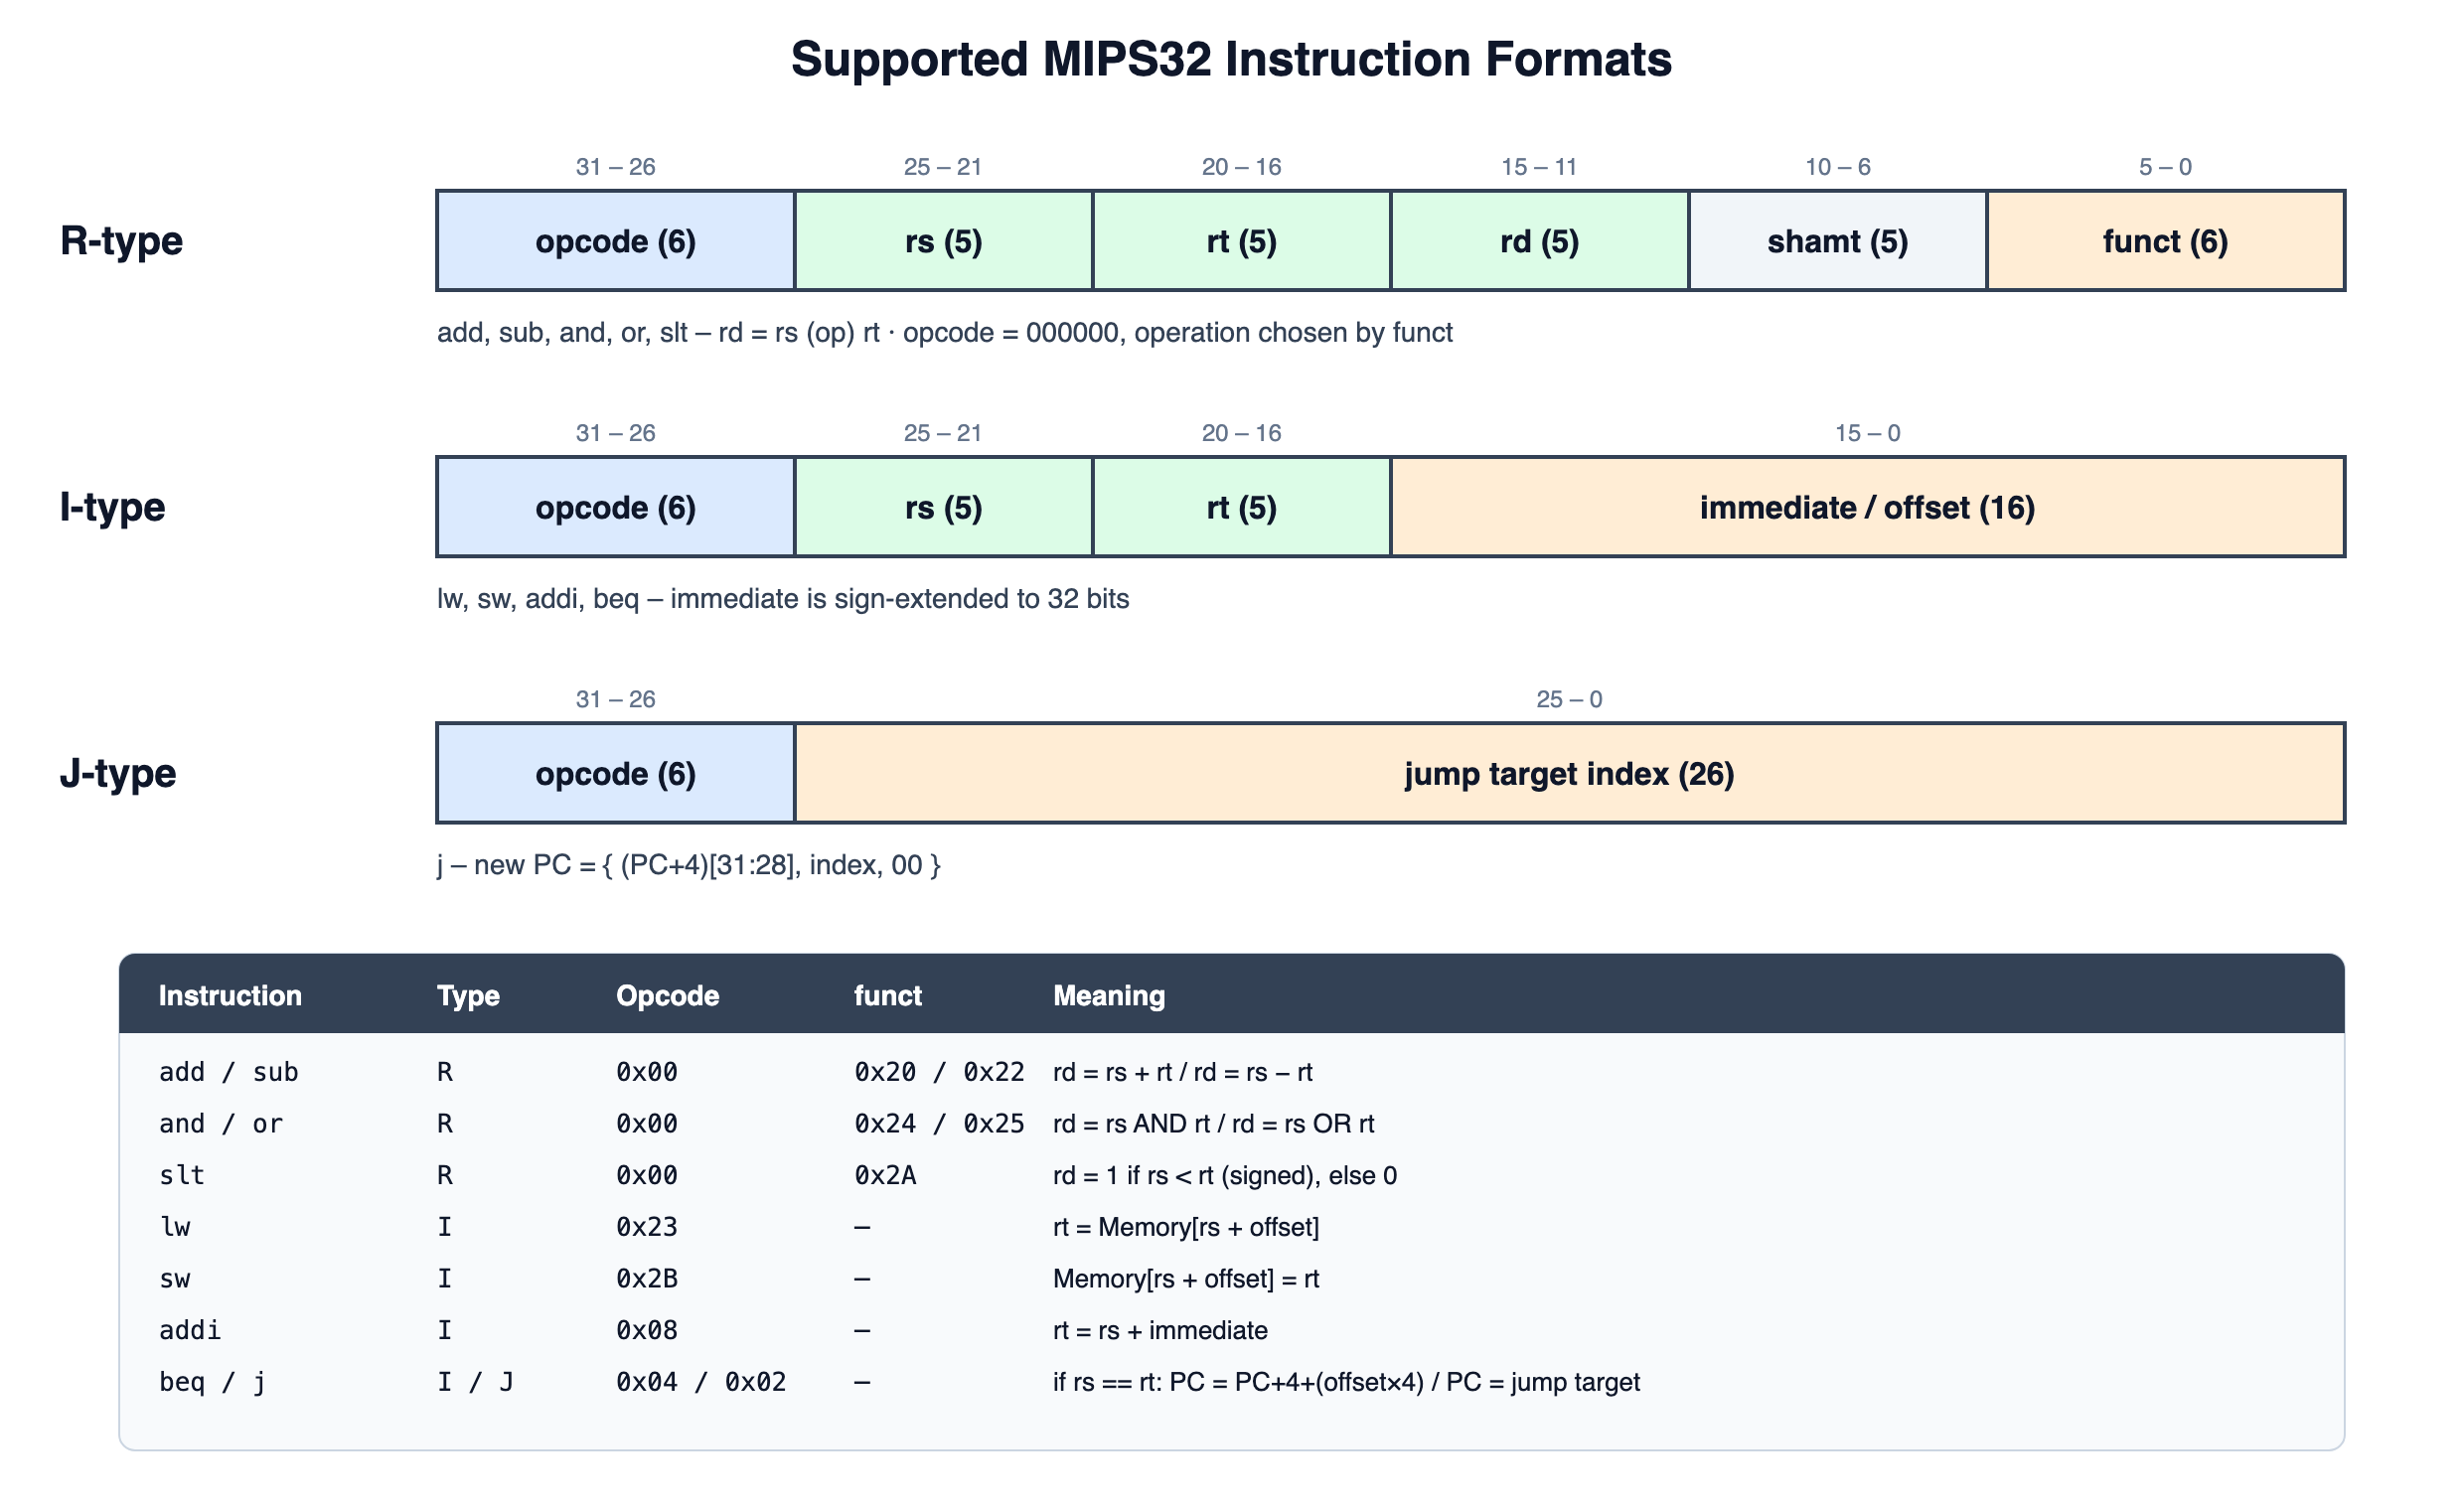
\includegraphics[width=\columnwidth]{03_instruction_formats.png}
\caption{R, I and J instruction formats used by the decoder.}
\label{fig:formats}
\end{figure}

\subsection{Datapath}
Fig.~\ref{fig:datapath} shows the complete datapath and control. On each
rising clock edge the program counter (\texttt{pc.v}) loads the next address.
The instruction ROM (\texttt{instruction\_memory.v}) is read combinationally
at the PC. Fields $rs$ and $rt$ address the two read ports of the register
file (\texttt{register\_file.v}); the RegDst multiplexer selects $rd$ (R-type)
or $rt$ (I-type) as the write register. The sign extender
(\texttt{sign\_extend.v}) widens the 16-bit immediate, and the ALUSrc
multiplexer selects it or $rt$ as the second ALU operand. The ALU
(\texttt{alu.v}) result is used as the data-memory address for \texttt{lw} and
\texttt{sw} or as the write-back value; the MemToReg multiplexer selects the
ALU result or the data read from memory. The branch/jump unit
(\texttt{branch\_jump.v}) computes $PC{+}4$, the branch target
$PC{+}4{+}(\mathrm{SE}(imm){\ll}2)$ and the jump target, and selects the next
PC with priority \emph{jump} $>$ \emph{branch taken} $>$ $PC{+}4$, where a
branch is taken when Branch $\wedge$ Zero.

\begin{figure*}[!tbp]
\centering
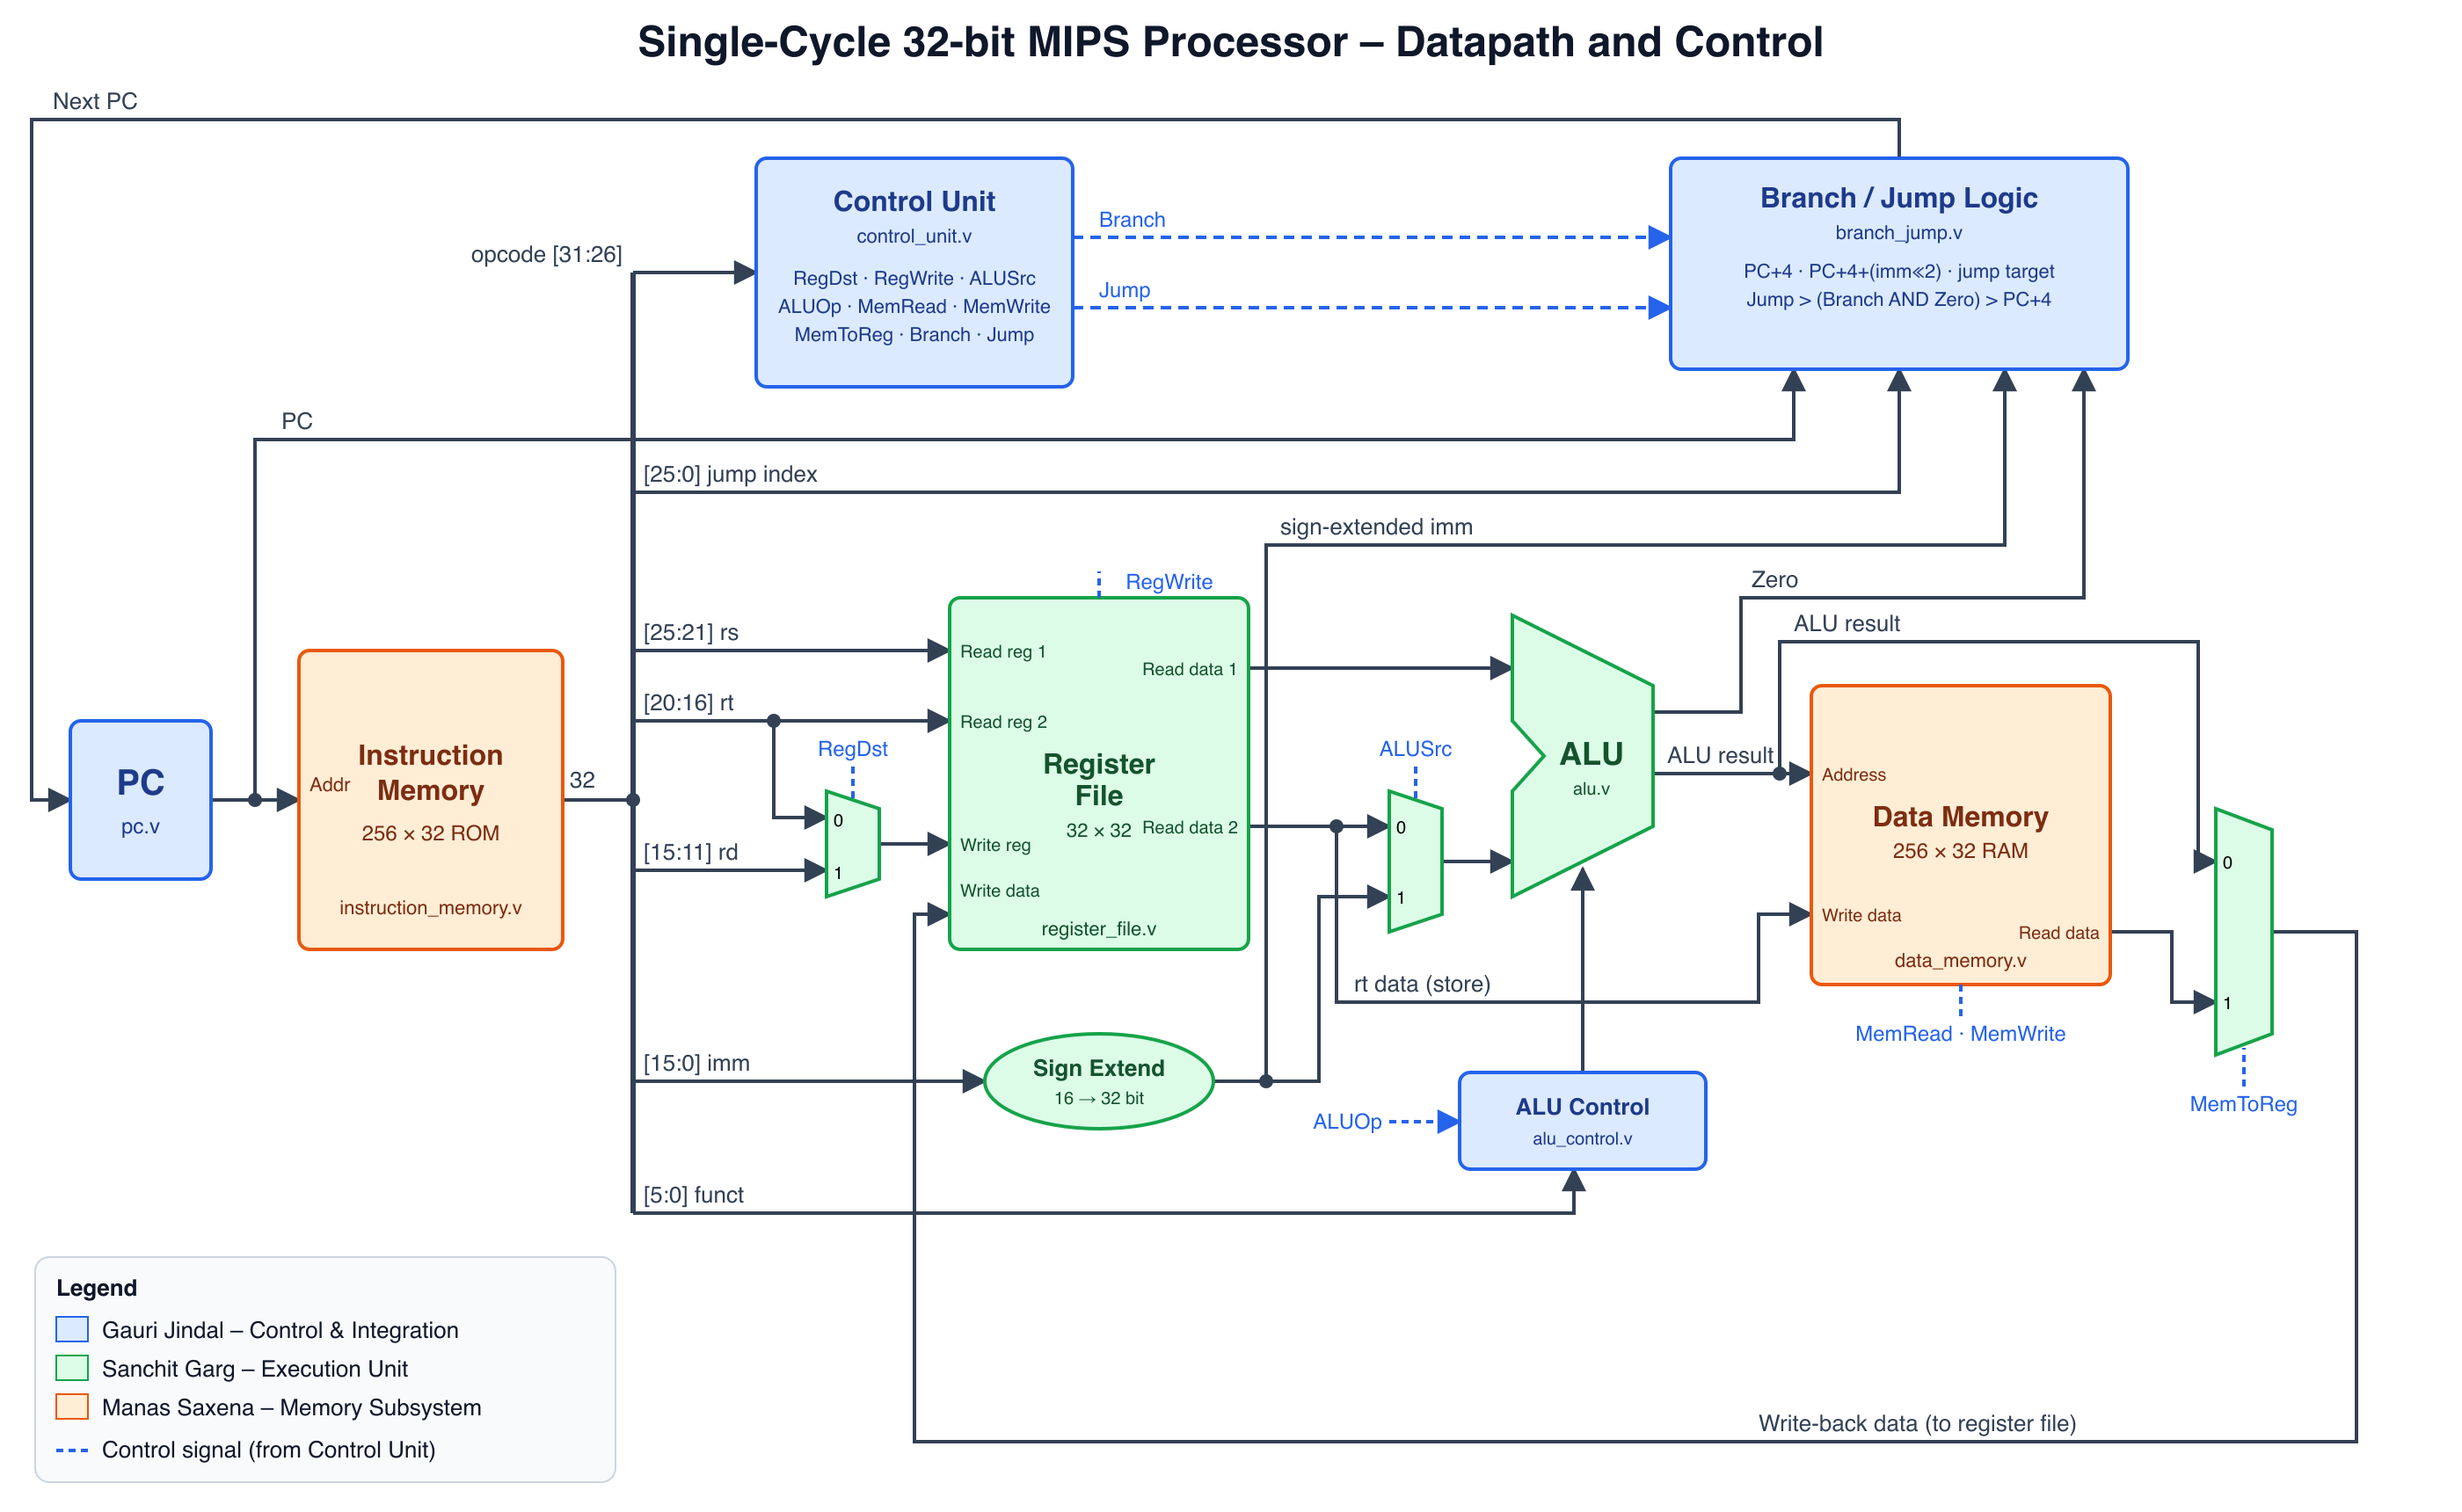
\includegraphics[width=0.82\textwidth]{01_datapath.png}
\caption{Single-cycle MIPS datapath and control, showing module boundaries.}
\label{fig:datapath}
\end{figure*}

\subsection{Control unit}
The main decoder (\texttt{control\_unit.v}) is a combinational function of the
6-bit opcode that produces nine control signals (Table~\ref{tab:control}).
All outputs default to zero, so an unsupported opcode behaves as a no-operation
that writes neither registers nor memory. The ALU decoder
(\texttt{alu\_control.v}) implements the classic two-level scheme: ALUOp
$=00$ selects ADD (address and \texttt{addi}), $01$ selects SUB (\texttt{beq}
comparison) and $10$ uses the funct field to choose ADD, SUB, AND, OR or SLT.

\begin{table}[!tbp]
\caption{Main control unit truth table}
\label{tab:control}
\centering
\footnotesize
\setlength{\tabcolsep}{3pt}
\resizebox{\columnwidth}{!}{\begin{tabular}{@{}lccccccccc@{}}
\toprule
Instr. & RegDst & RegWr & ALUSrc & ALUOp & MemRd & MemWr & MemToReg & Br & J \\
\midrule
R-type & 1 & 1 & 0 & 10 & 0 & 0 & 0 & 0 & 0 \\
\texttt{lw}   & 0 & 1 & 1 & 00 & 1 & 0 & 1 & 0 & 0 \\
\texttt{sw}   & x & 0 & 1 & 00 & 0 & 1 & x & 0 & 0 \\
\texttt{addi} & 0 & 1 & 1 & 00 & 0 & 0 & 0 & 0 & 0 \\
\texttt{beq}  & x & 0 & 0 & 01 & 0 & 0 & x & 1 & 0 \\
\texttt{j}    & x & 0 & x & xx & 0 & 0 & x & 0 & 1 \\
\bottomrule
\end{tabular}}
\end{table}

\subsection{Execution unit}
The register file contains 32 registers of 32 bits with two asynchronous read
ports and one synchronous write port. Writes to \texttt{\$zero} are ignored and
reads of \texttt{\$zero} return 0. The ALU supports AND, OR, ADD, SUB and
signed SLT (using \texttt{\$signed} comparison) and produces a Zero flag used
by \texttt{beq}. The sign extender replicates bit 15 of the immediate.

\subsection{Memory interface}
The memory subsystem follows a Harvard organization (Fig.~\ref{fig:memory}).
Both memories hold $256\times32$-bit words (1~KB) and use byte addresses with
word index $address[9{:}2]$. An access is valid only if
$address[31{:}10]=0$ and $address[1{:}0]=00$; invalid instruction fetches
return a NOP, invalid reads return 0 and invalid writes are ignored. The
instruction ROM is initialized from \texttt{programs/instruction\_memory.mem}
with \texttt{\$readmemh}. The data RAM has a combinational read gated by
MemRead and a synchronous write gated by MemWrite. One active-high synchronous
reset is distributed from the CPU to the PC, register file and data memory, so
a single reset returns the whole processor to a known state.

\begin{figure}[!tbp]
\centering
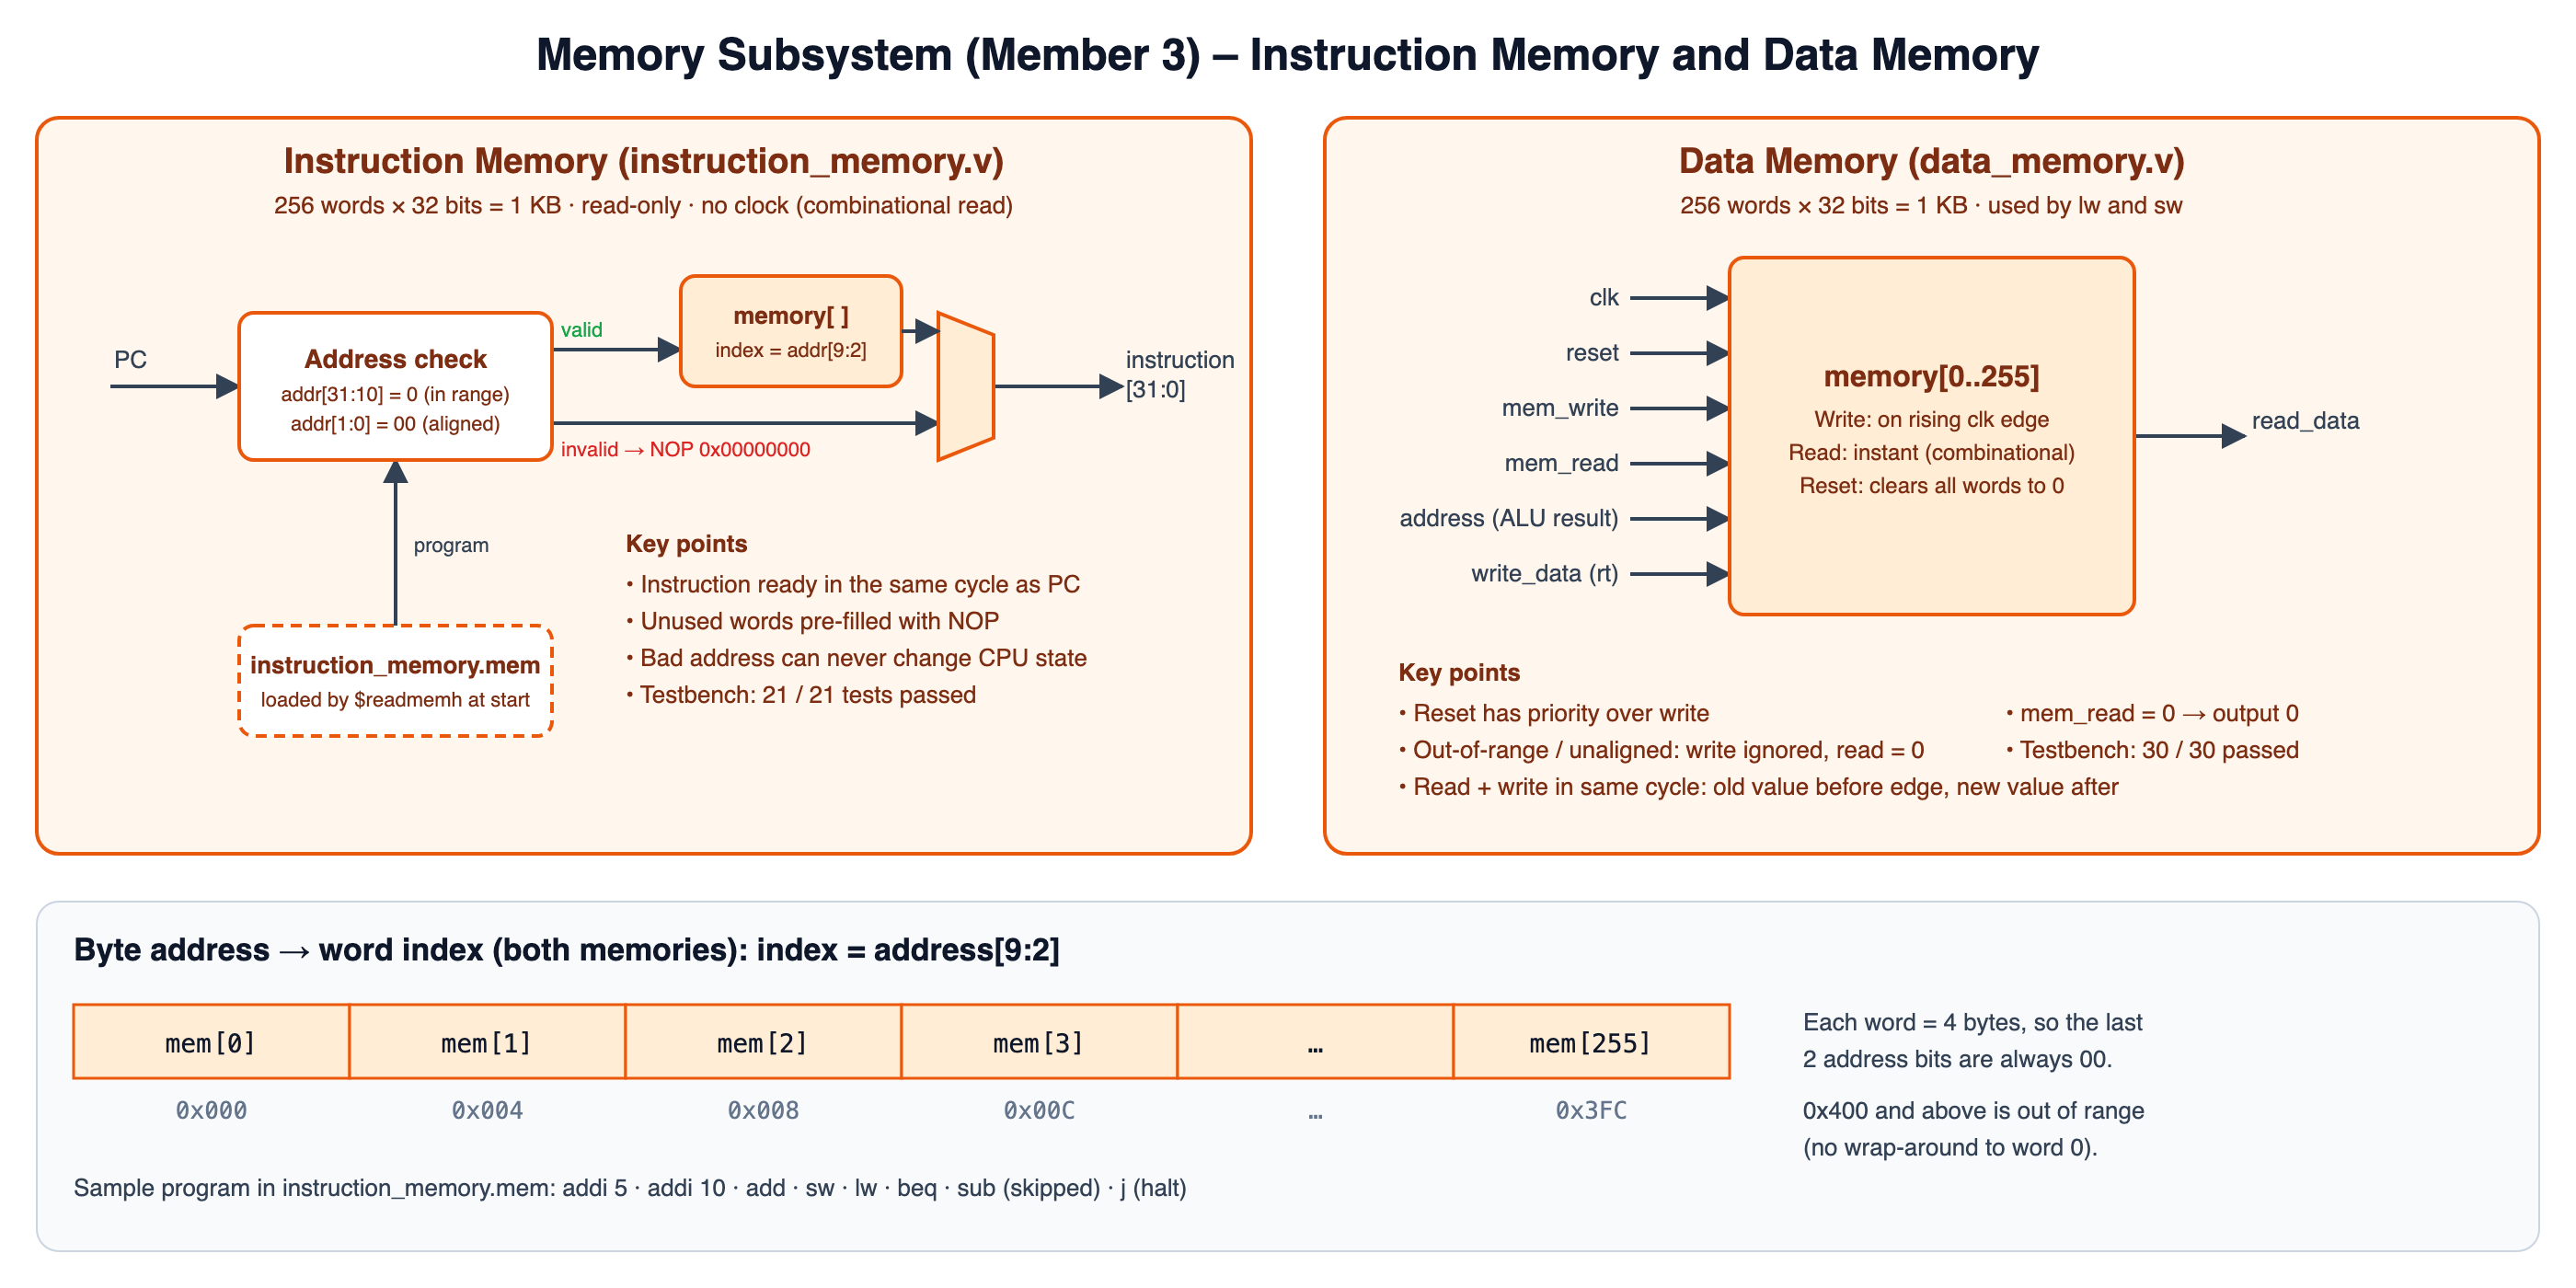
\includegraphics[width=\columnwidth]{06_memory_subsystem.png}
\caption{Harvard memory subsystem: instruction ROM and data RAM with address
validation.}
\label{fig:memory}
\end{figure}

\subsection{Verification methodology}
Verification is bottom-up (Fig.~\ref{fig:verif}). Each module has a
self-checking testbench that applies directed vectors, compares the result
with an expected value and prints PASS/FAIL. The CPU testbench writes
hand-assembled machine code directly into the instruction ROM, runs each
program for a fixed number of cycles and checks registers and data memory. It
also checks, before every program, that the hardware reset cleared the PC, all
registers and all 256 data words. A separate performance testbench counts the
dynamic instruction mix until each program reaches its halt loop
(\texttt{j} to itself). All simulations use Icarus Verilog~\cite{icarus} and
produce VCD waveforms.

\begin{figure}[!tbp]
\centering
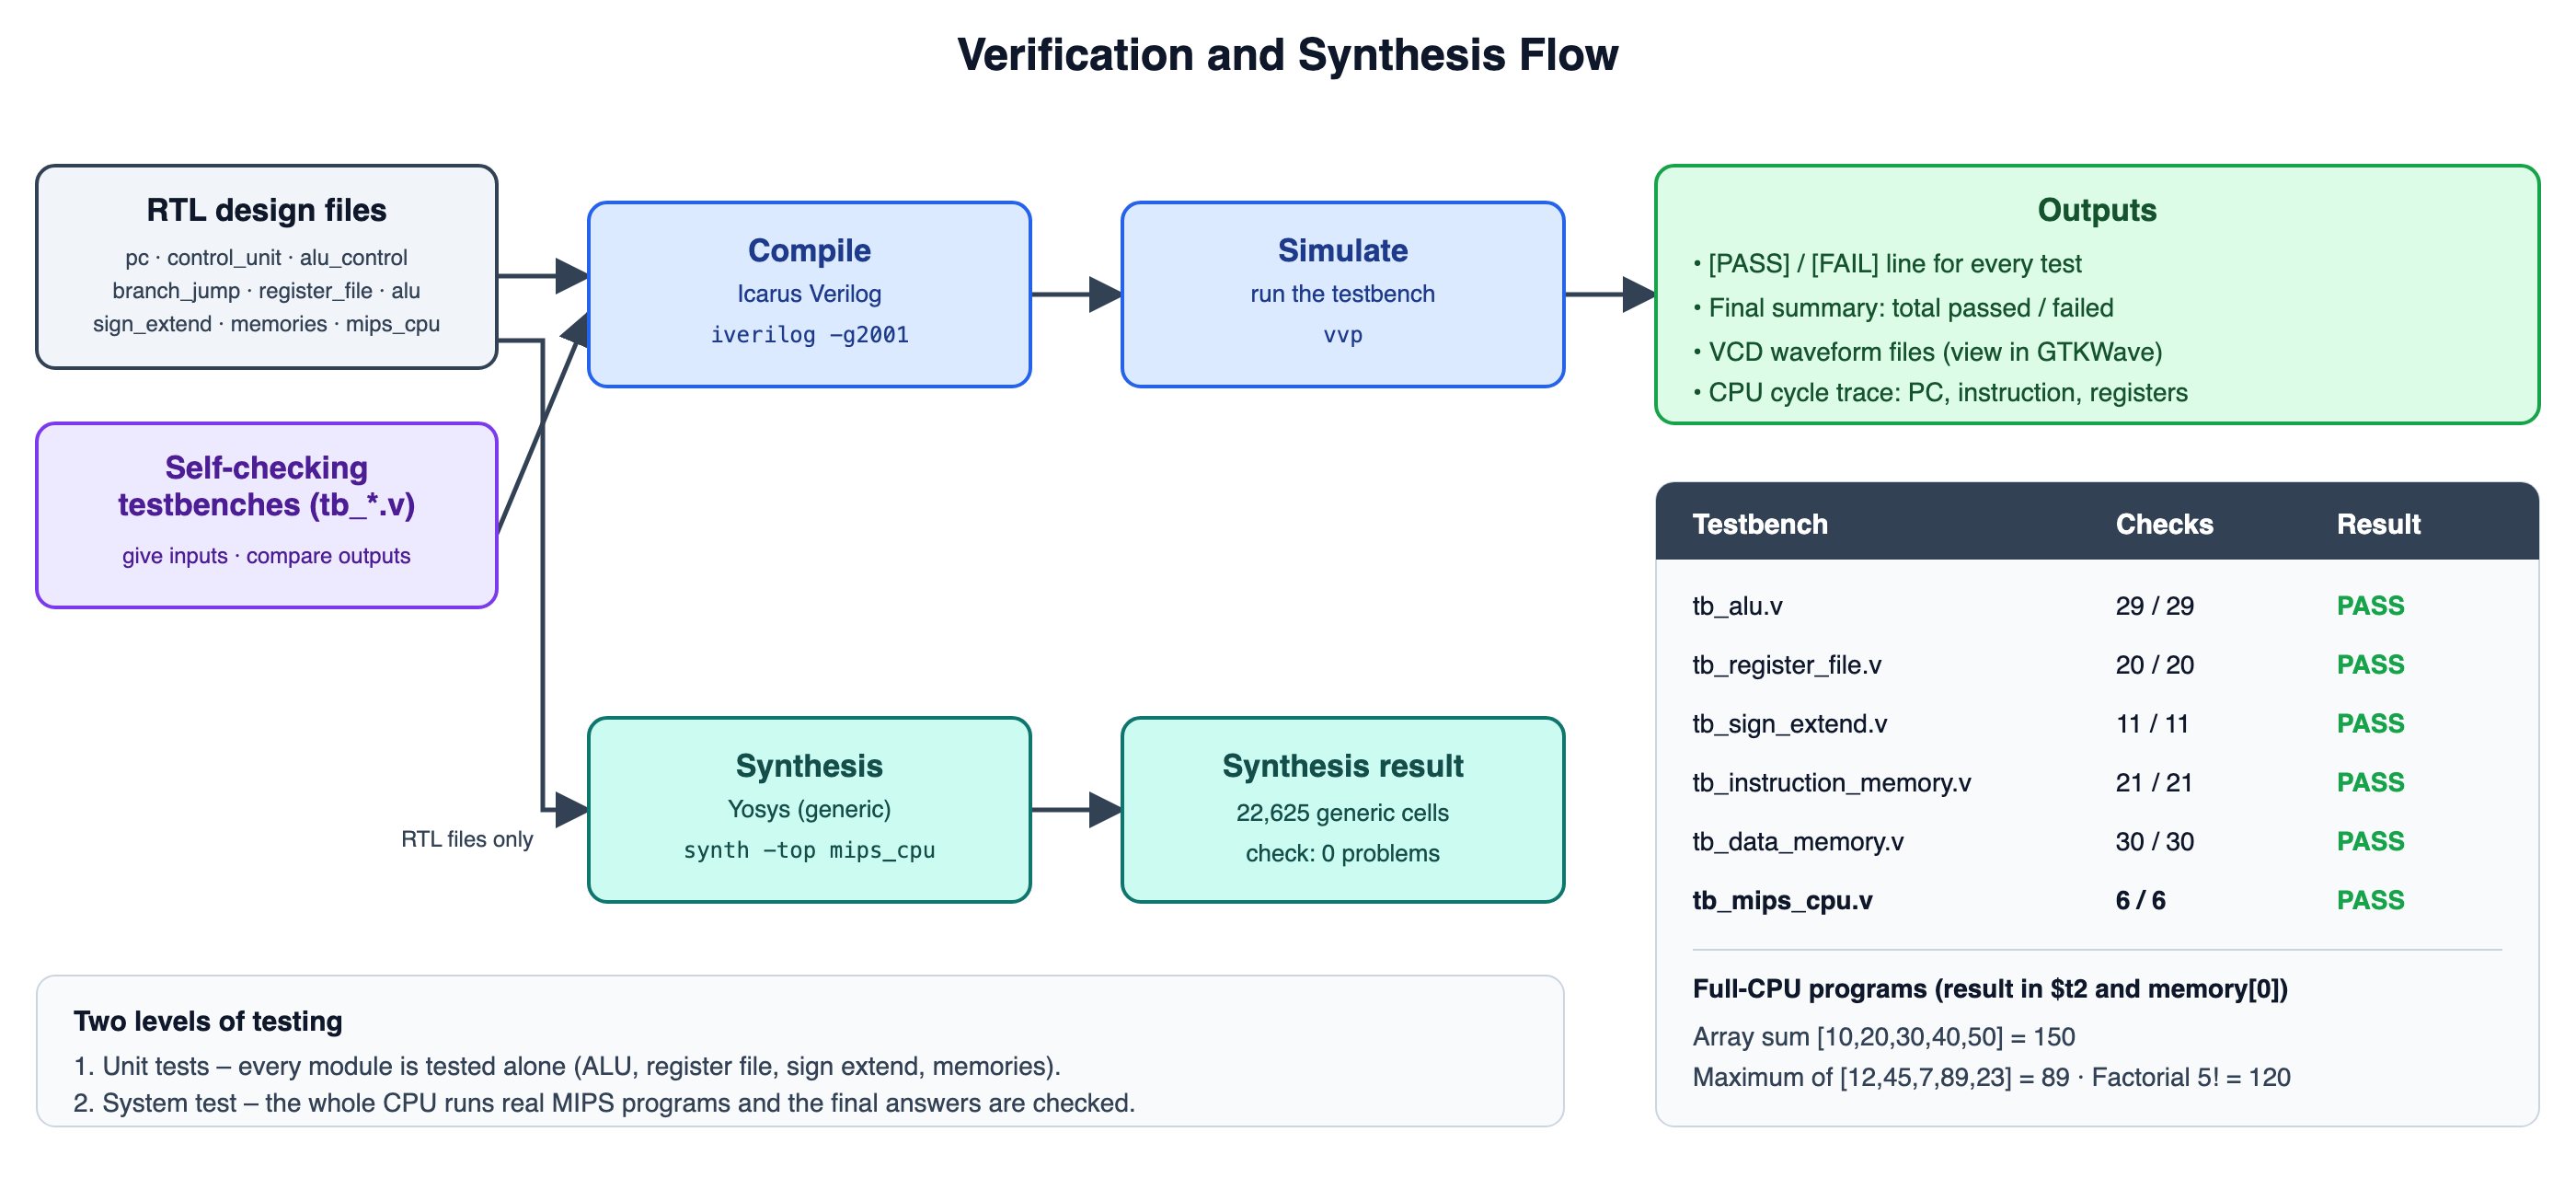
\includegraphics[width=\columnwidth]{07_verification_flow.png}
\caption{Verification and synthesis flow.}
\label{fig:verif}
\end{figure}

\subsection{Test programs}
Four programs exercise every instruction:
\begin{enumerate}
  \item \textbf{Array sum} of $[10,20,30,40,50]$ using \texttt{addi},
        \texttt{add}, \texttt{sw} and \texttt{j}; expected 150.
  \item \textbf{Maximum search} over $[12,45,7,89,23]$ using \texttt{slt} and
        \texttt{beq} to skip the update; expected 89.
  \item \textbf{Factorial} $5!$ computed with nested loops of repeated
        addition (no multiplier), using \texttt{beq}, \texttt{slt} and
        \texttt{j}; expected 120.
  \item \textbf{Jump/logic test}: \texttt{j} skips an \texttt{addi} that must
        not execute, followed by \texttt{sub}, \texttt{and}, \texttt{or},
        \texttt{slt}, \texttt{sw} and \texttt{lw} at address 4.
\end{enumerate}

\subsection{Synthesis flow}
The RTL is synthesized with Yosys~\cite{yosys} for a Xilinx 7-series target to
estimate LUT and flip-flop usage, and with Yosys and nextpnr~\cite{shah2019yosys}
for a Gowin GW5AST-138 FPGA (Sipeed Tang Mega 138K Pro) to obtain a placed
design with static timing analysis. A board wrapper
(\texttt{synthesis/fpga\_top.v}) folds the 64 debug output bits into six LEDs
using XOR so that no CPU logic is removed by optimization. A Vivado script and
Basys3 constraints are also provided for the Xilinx vendor flow.

% ============================================================================
\section{Results and Discussion}

\subsection{Functional verification}
Table~\ref{tab:tests} summarizes the simulation results. All 129 directed
checks pass. Every program produces the expected result in register
\texttt{\$t2} and in data memory.

\begin{table}[!tbp]
\caption{Simulation results (Icarus Verilog 13.0)}
\label{tab:tests}
\centering
\footnotesize
\resizebox{\columnwidth}{!}{\begin{tabular}{@{}lll@{}}
\toprule
Testbench & Coverage & Result \\
\midrule
\texttt{tb\_alu} & all ops, Zero, signed SLT, overflow & 29/29 \\
\texttt{tb\_register\_file} & R/W, reset, \texttt{\$zero}, all regs & 20/20 \\
\texttt{tb\_sign\_extend} & positive/negative, boundaries & 11/11 \\
\texttt{tb\_instruction\_memory} & fetch, init, invalid/unaligned & 21/21 \\
\texttt{tb\_data\_memory} & R/W, reset, invalid, R-before-W & 30/30 \\
\texttt{tb\_mips\_cpu} & 4 programs + 5 reset checks & 18/18 \\
\midrule
\multicolumn{2}{@{}l}{\textbf{Total}} & \textbf{129/129} \\
\bottomrule
\end{tabular}}
\end{table}

\begin{table}[!tbp]
\caption{Program results}
\label{tab:programs}
\centering
\footnotesize
\resizebox{\columnwidth}{!}{\begin{tabular}{@{}lll@{}}
\toprule
Program & Expected & Observed \\
\midrule
Array sum $[10,\dots,50]$ & \$t2 = MEM[0] = 150 & 150 \\
Maximum $[12,45,7,89,23]$ & \$t2 = MEM[0] = 89 & 89 \\
Factorial $5!$ & \$t2 = MEM[0] = 120 & 120 \\
Jump/logic & 2, 8, 14, 1, MEM[4]=14, 14 & all match \\
\bottomrule
\end{tabular}}
\end{table}

\subsection{Waveform analysis}
Figs.~\ref{fig:wsum}--\ref{fig:wreset} are taken from the VCD files of the CPU
testbench. In the array sum (Fig.~\ref{fig:wsum}) each \texttt{add} updates
\texttt{\$t2} on the rising edge (30, 60, 100, 150); while the PC is 0x24 the
\texttt{sw} asserts MemWrite with RegWrite low and MEM[0] becomes 150 on the
next edge. In the maximum search (Fig.~\ref{fig:wmax}) \texttt{beq} is taken
when \texttt{slt} returns 0, so next-PC skips the update instruction; the
maximum changes only for 45 and 89. The factorial (Fig.~\ref{fig:wfact}) shows
the outer counter \texttt{\$t0} decrementing from 5 to 0 while \texttt{\$t2}
takes the values 1, 5, 20, 60 and 120. In the jump test (Fig.~\ref{fig:wjump})
the \texttt{j} at 0x08 changes the PC directly to 0x10, so the instruction at
0x0C never executes; MemWrite and MemRead show the store of 14 to address 4 and
the load that reads it back. Fig.~\ref{fig:wreset} confirms that one reset
pulse clears the PC, the register file and the data memory. Fig.~\ref{fig:walu}
shows the ALU unit test, including signed SLT and the Zero flag.

\begin{figure*}[!tbp]
\centering
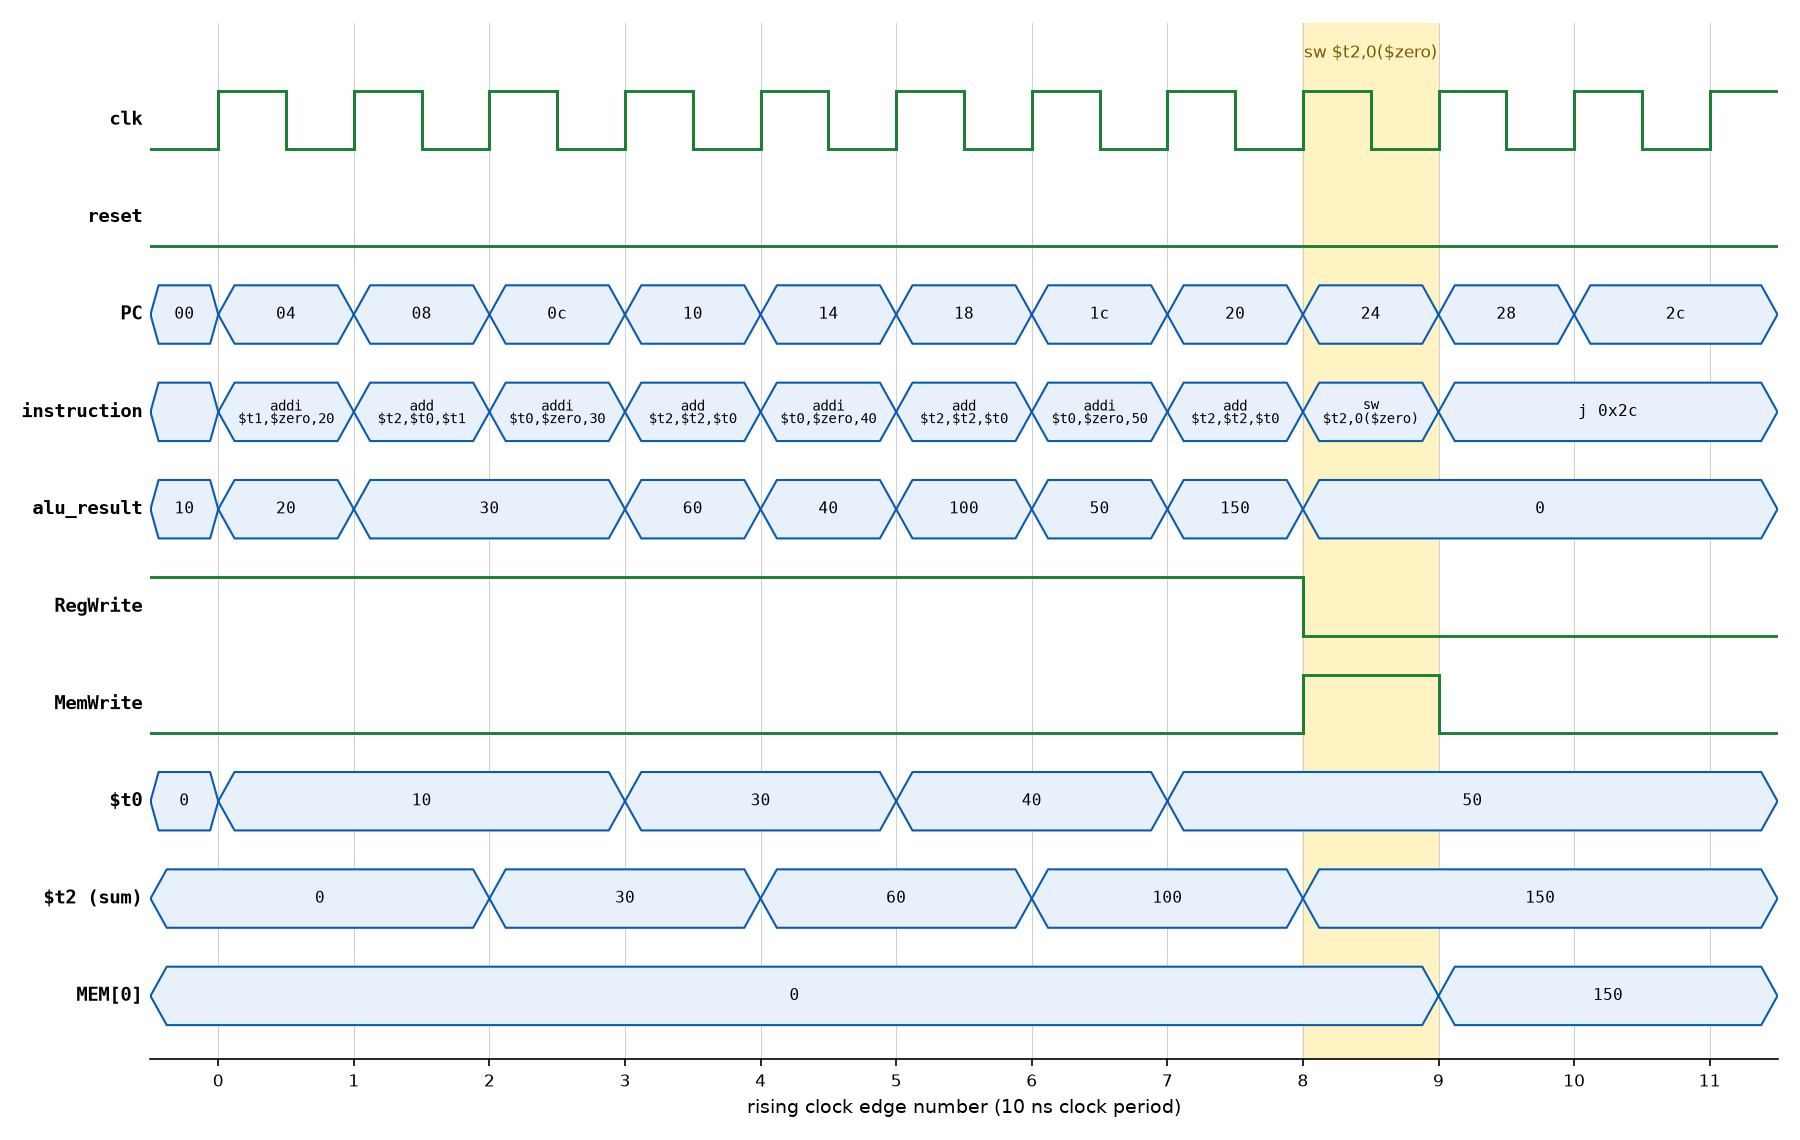
\includegraphics[width=0.9\textwidth]{01_array_sum.png}
\caption{Array-sum execution: PC, disassembled instruction, ALU result,
control signals, registers and data memory.}
\label{fig:wsum}
\end{figure*}

\begin{figure*}[!tbp]
\centering
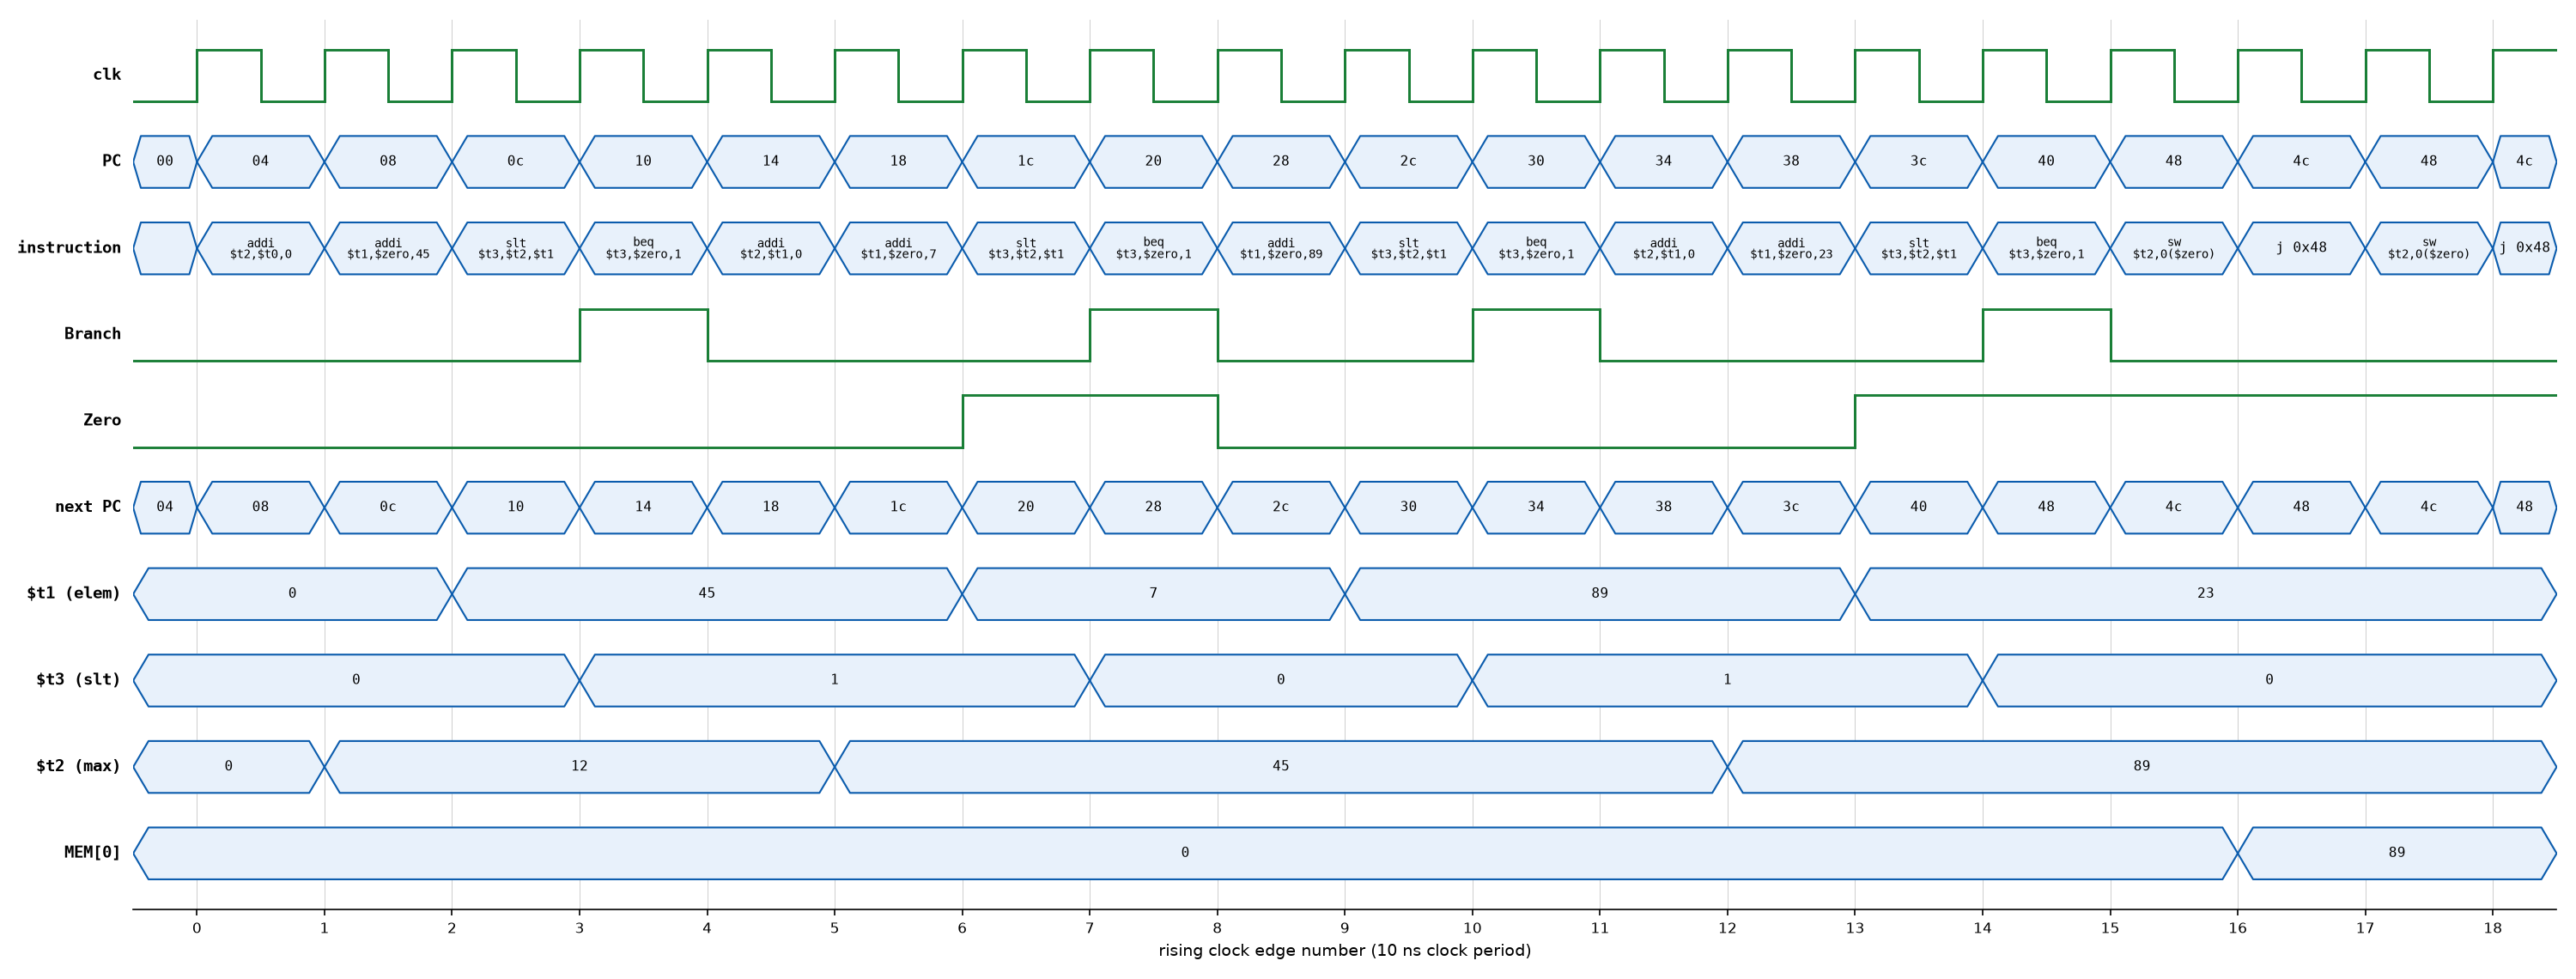
\includegraphics[width=\textwidth]{02_max_search.png}
\caption{Maximum search: \texttt{beq} redirects the next PC when the new
element is not larger.}
\label{fig:wmax}
\end{figure*}

\begin{figure*}[!tbp]
\centering
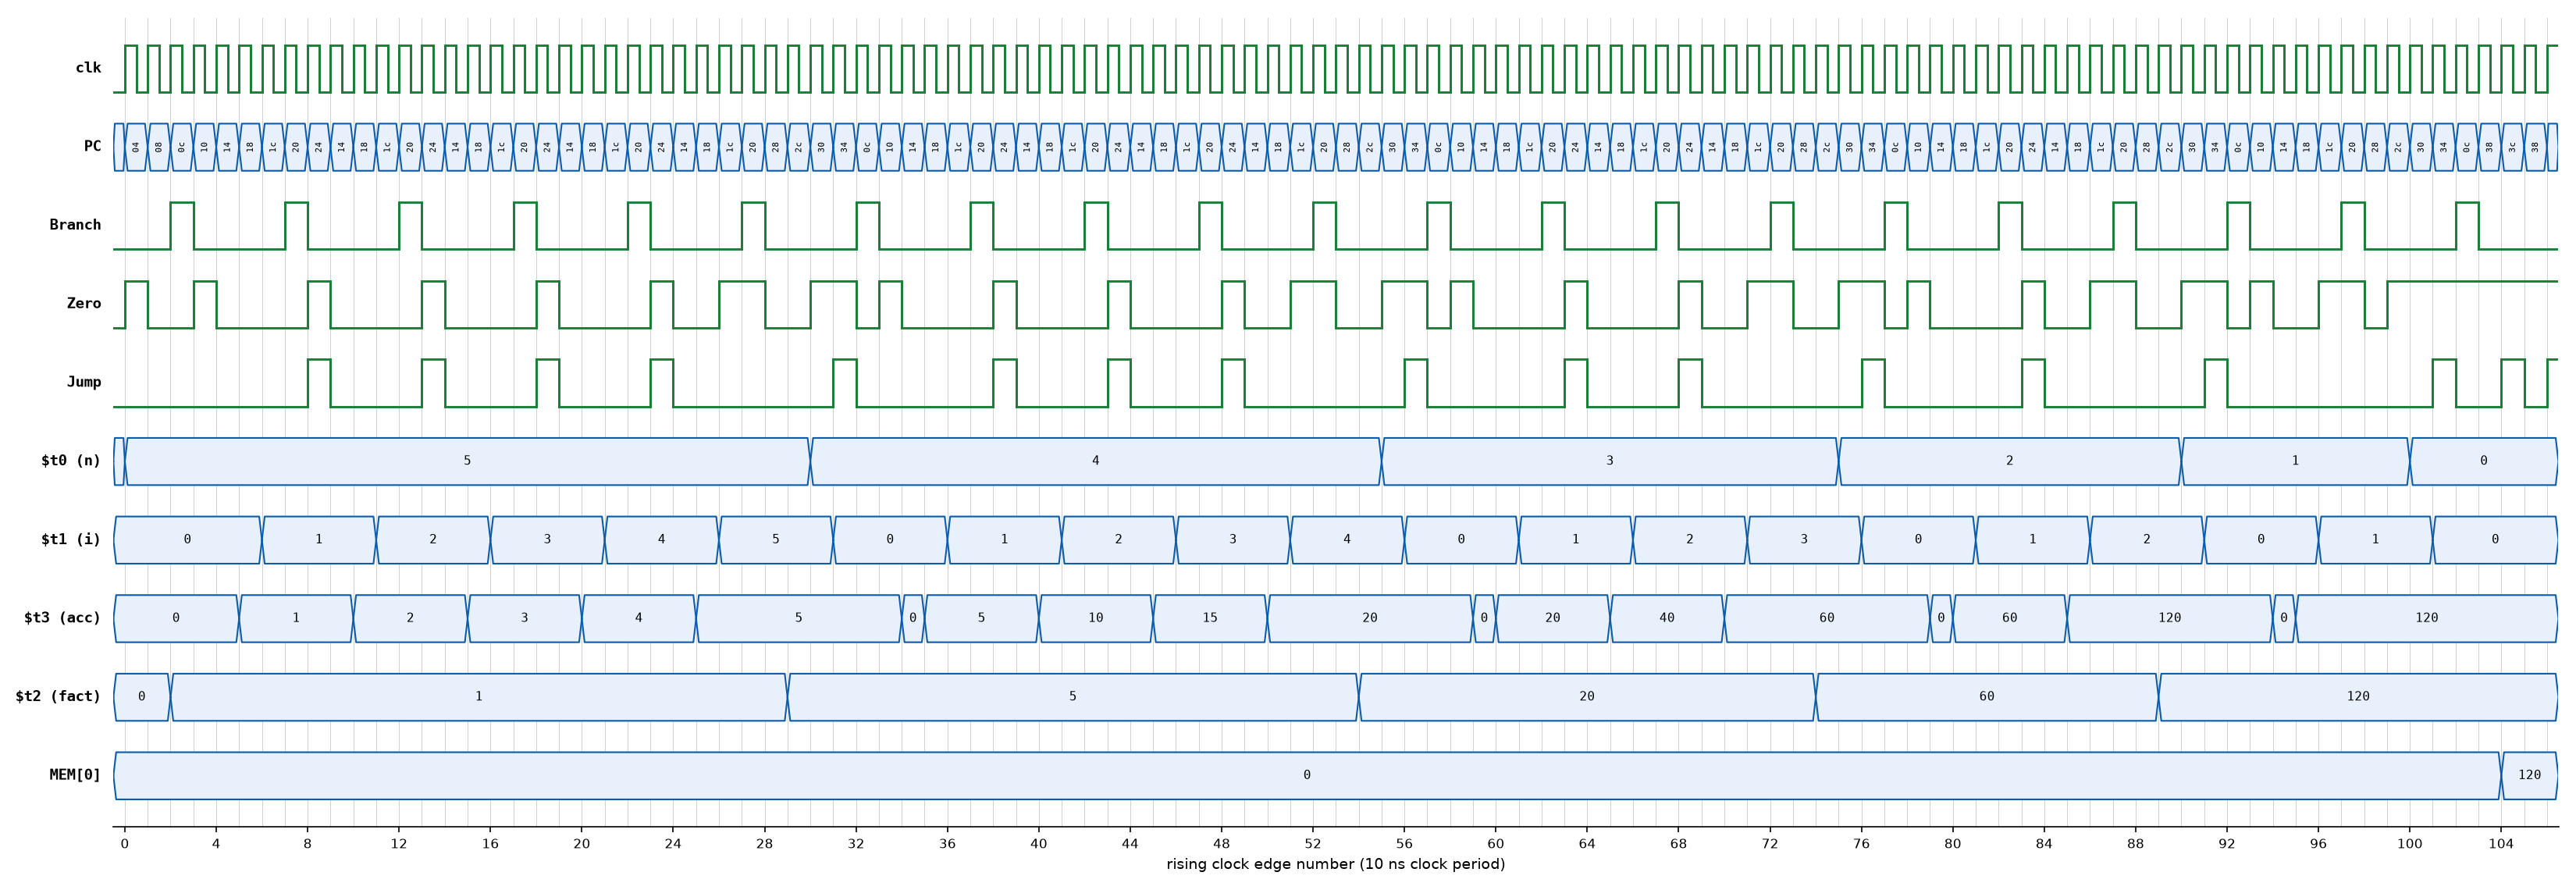
\includegraphics[width=\textwidth]{03_factorial.png}
\caption{Factorial $5!$ (106 cycles): branch, jump and loop counters.}
\label{fig:wfact}
\end{figure*}

\begin{figure*}[!tbp]
\centering
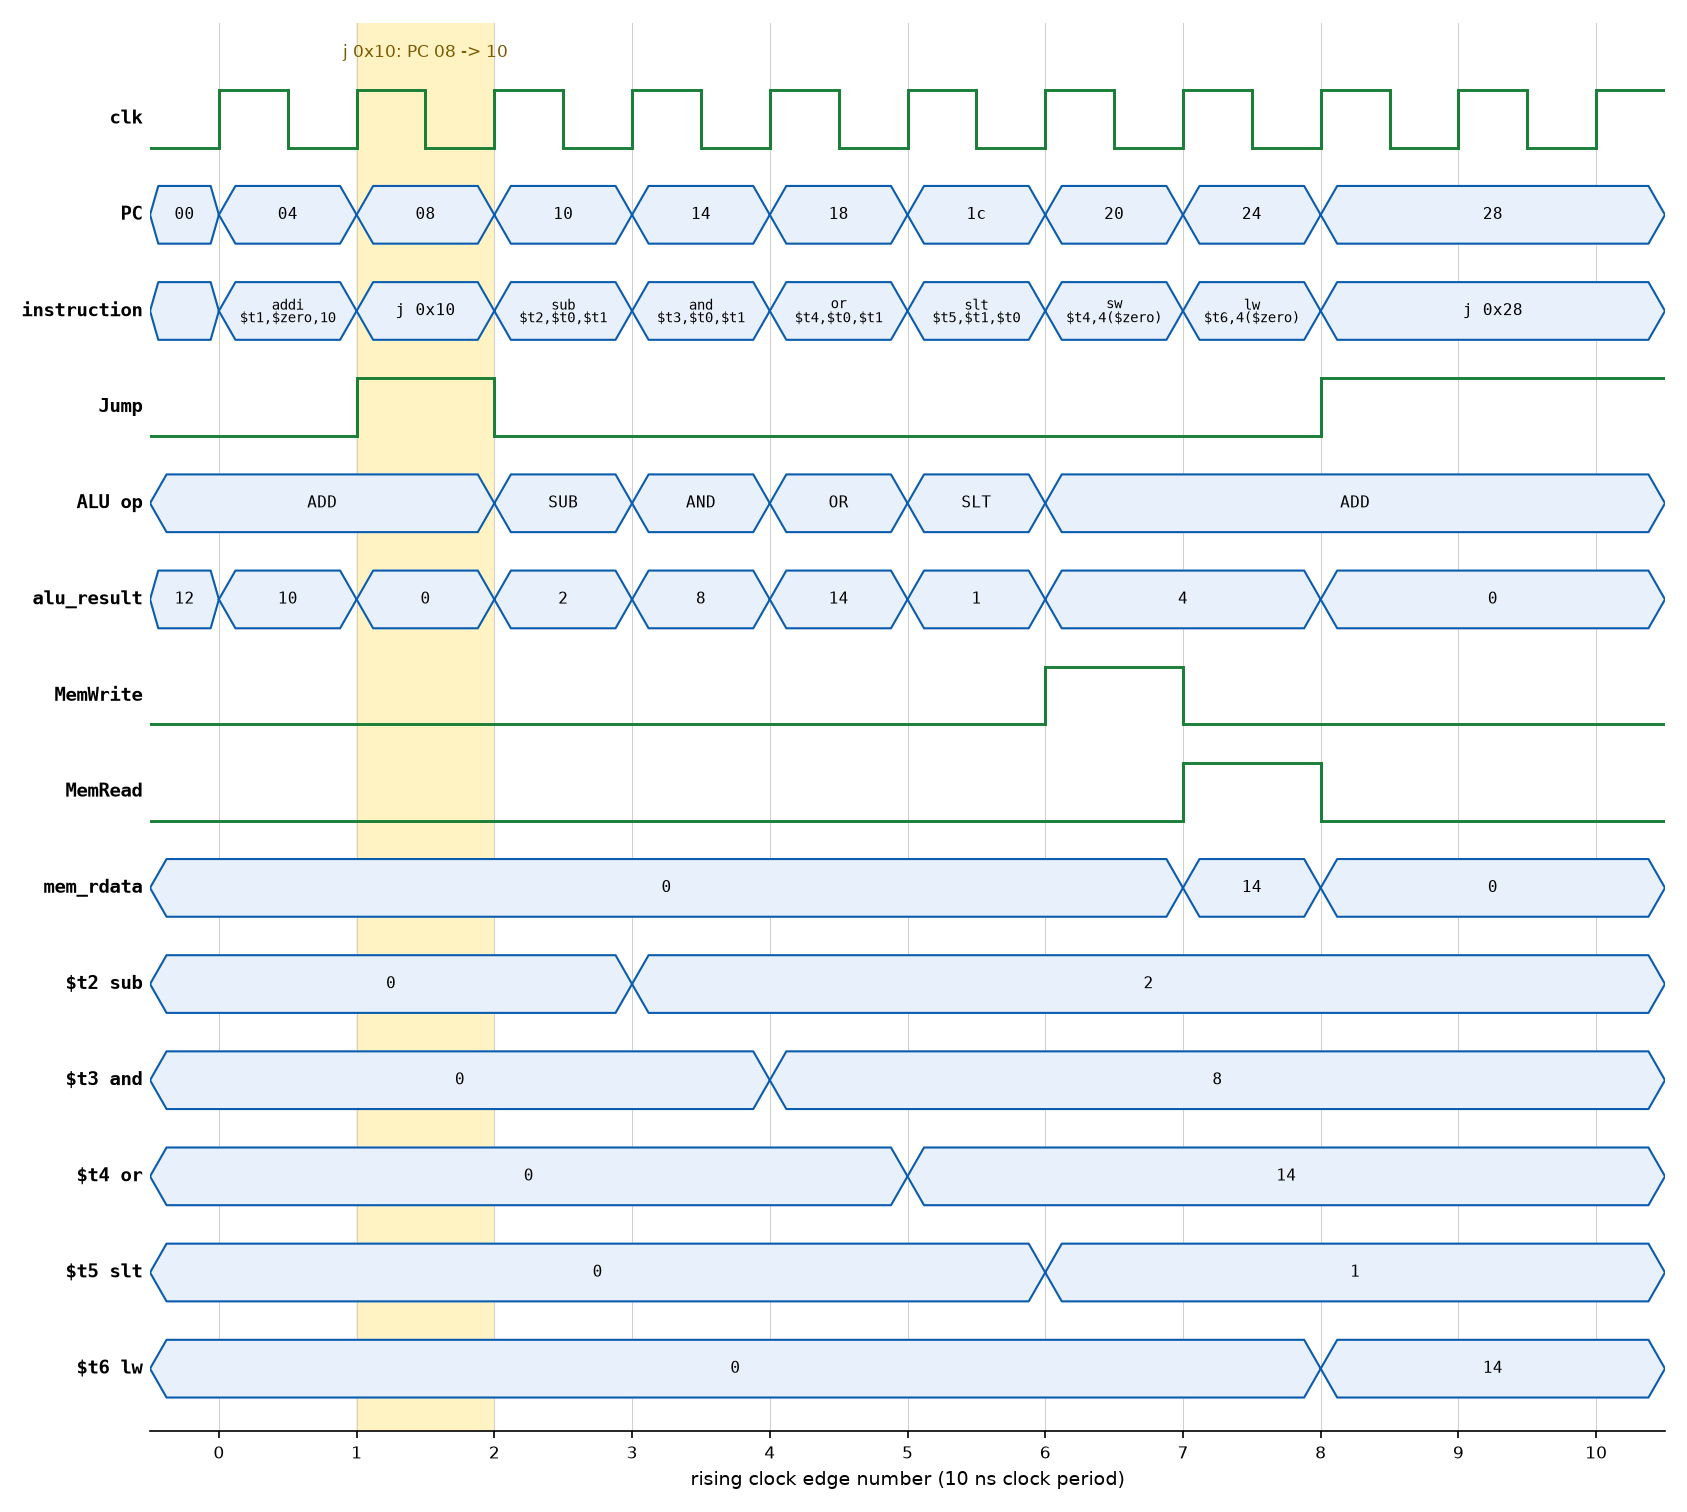
\includegraphics[width=0.85\textwidth]{04_jump_logic.png}
\caption{Jump/logic test: \texttt{j} skips 0x0C; SUB/AND/OR/SLT results and
SW/LW at address 4.}
\label{fig:wjump}
\end{figure*}

\begin{figure}[!tbp]
\centering
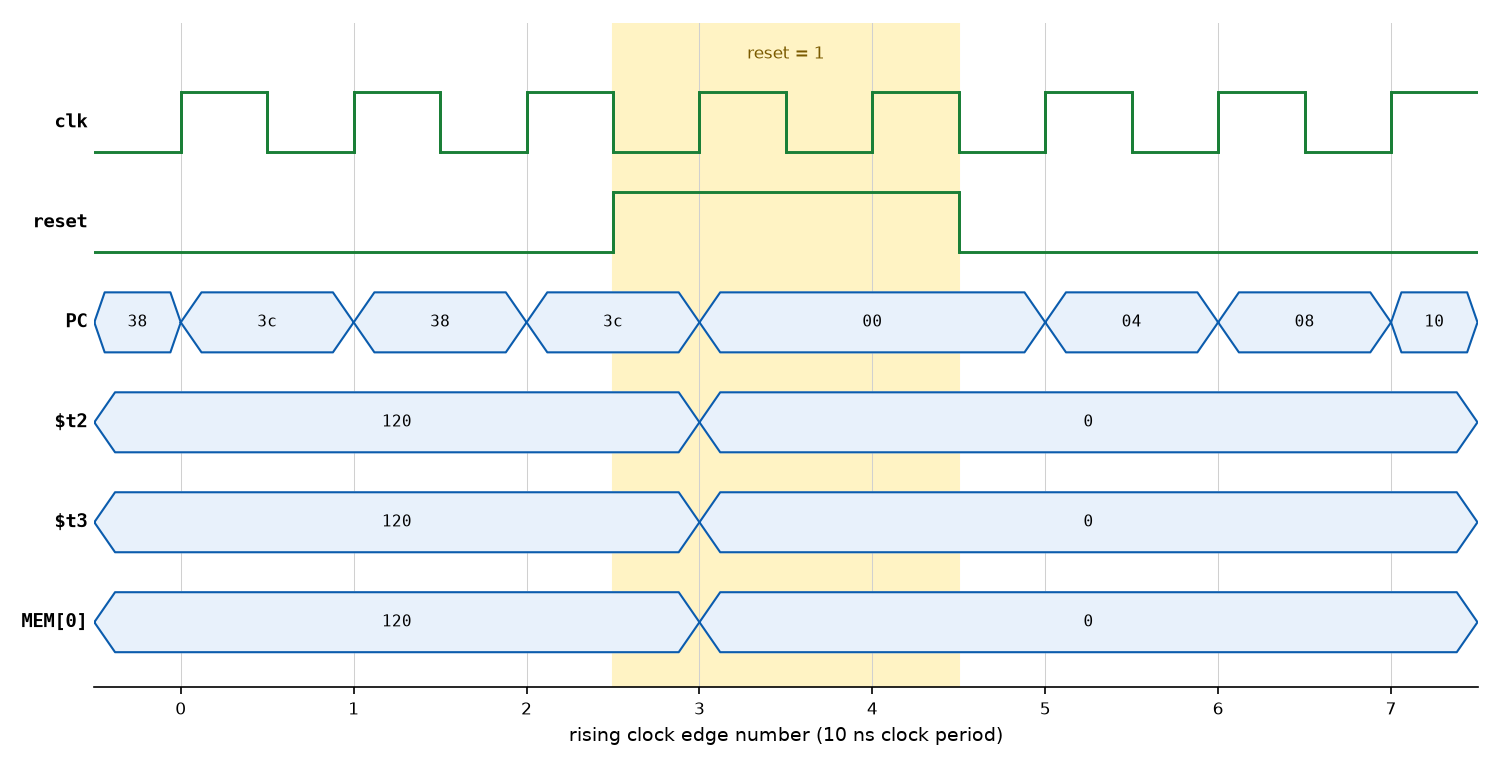
\includegraphics[width=\columnwidth]{05_reset.png}
\caption{Synchronous reset between two programs.}
\label{fig:wreset}
\end{figure}

\begin{figure*}[!tbp]
\centering
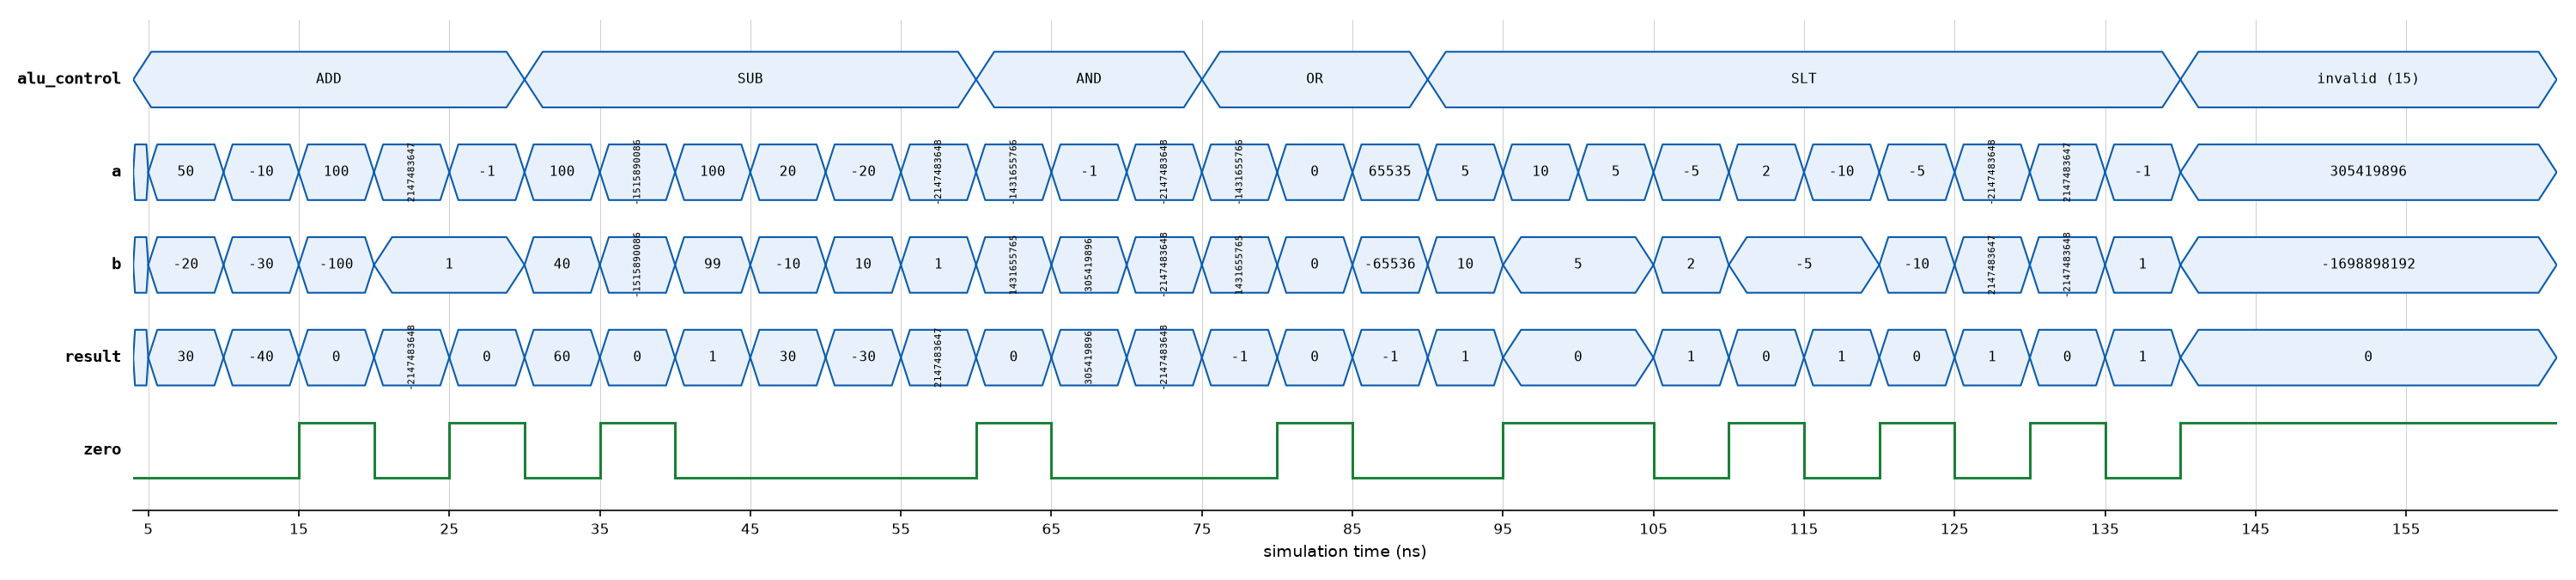
\includegraphics[width=\textwidth]{06_alu.png}
\caption{ALU testbench waveform (signed decimal values).}
\label{fig:walu}
\end{figure*}

\subsection{Performance}
The performance testbench counts the dynamic instruction mix of each program
(Table~\ref{tab:perf}). The single-cycle CPU executes one instruction per
cycle, so CPI~$=1.00$ exactly. For comparison, the same mix on the classic
multi-cycle MIPS (R-type and \texttt{addi} 4 cycles, \texttt{lw} 5,
\texttt{sw} 4, \texttt{beq} and \texttt{j} 3)~\cite{patterson2014cod} needs
527 cycles, an average CPI of 3.71.

Execution time depends on the clock period as well as CPI. With the textbook
component delays (memory 200~ps, register read 100~ps, ALU 200~ps, register
write 100~ps) the single-cycle clock must cover the \texttt{lw} path,
$200{+}100{+}200{+}200{+}100=800$~ps, while the multi-cycle clock needs only
200~ps. The resulting total times are 113.6~ns (single-cycle) and 105.4~ns
(multi-cycle): the multi-cycle design is about 7\% faster on this workload
because most instructions are R-type, \texttt{addi} and \texttt{beq}, which
do not use data memory. This quantifies the main weakness of the single-cycle
organization -- every instruction pays for the slowest one -- and motivates
pipelining, which keeps CPI near 1 at a short clock period.

\begin{table}[!tbp]
\caption{Dynamic instruction count, cycles and CPI}
\label{tab:perf}
\centering
\footnotesize
\setlength{\tabcolsep}{3pt}
\resizebox{\columnwidth}{!}{\begin{tabular}{@{}lrrrrrr@{}}
\toprule
& & \multicolumn{2}{c}{Single-cycle} & \multicolumn{3}{c}{Multi-cycle} \\
\cmidrule(lr){3-4}\cmidrule(l){5-7}
Program & Instr. & Cyc. & Time & Cyc. & CPI & Time \\
\midrule
Array sum  & 11  & 11  & 8.8 ns   & 43  & 3.90 & 8.6 ns \\
Max search & 17  & 17  & 13.6 ns  & 64  & 3.76 & 12.8 ns \\
Factorial  & 105 & 105 & 84.0 ns  & 384 & 3.65 & 76.8 ns \\
Jump/logic & 9   & 9   & 7.2 ns   & 36  & 4.00 & 7.2 ns \\
\midrule
\textbf{Total} & \textbf{142} & \textbf{142} & \textbf{113.6 ns} & \textbf{527} & \textbf{3.71} & \textbf{105.4 ns} \\
\bottomrule
\end{tabular}}
\end{table}

\subsection{Synthesis results}
Yosys reports no structural problems (\texttt{check}: 0 problems). Table~\ref{tab:xilinx}
gives the Artix-7 estimate. The flip-flop count is exactly
$8{,}192$ (data memory, $256\times32$) $+ 992$ (registers \texttt{\$1}--\texttt{\$31};
\texttt{\$0} is constant) $+ 32$ (PC) $=9{,}216$. Table~\ref{tab:gowin} gives the
Gowin results and the maximum frequency from nextpnr static timing analysis
after full routing. The 50~MHz target is just missed; the critical path is
20.74~ns (8.84~ns of logic and 11.90~ns of routing). The CPU was not run on a
board.

\begin{table}[!tbp]
\caption{Xilinx Artix-7 (xc7a35t) resource estimate, Yosys}
\label{tab:xilinx}
\centering
\footnotesize
\resizebox{\columnwidth}{!}{\begin{tabular}{@{}lrrr@{}}
\toprule
Resource & Used & Available & Util. \\
\midrule
LUTs (LUT2--LUT6) & 4{,}190 & 20{,}800 & 20.1\% \\
Flip-flops (FDRE) & 9{,}216 & 41{,}600 & 22.2\% \\
CARRY4 & 35 & 8{,}150 & 0.4\% \\
Block RAM & 0 & 50 & 0\% \\
\midrule
\multicolumn{4}{@{}l}{Cells by module: data memory 11{,}241; register file 1{,}825;} \\
\multicolumn{4}{@{}l}{ALU 183; branch/jump 80; PC 32; control 13.} \\
\bottomrule
\end{tabular}}
\end{table}

\begin{table}[!tbp]
\caption{Gowin GW5AST-138 place-and-route results (nextpnr)}
\label{tab:gowin}
\centering
\footnotesize
\resizebox{\columnwidth}{!}{\begin{tabular}{@{}lrrr@{}}
\toprule
Resource & Used & Available & Util. \\
\midrule
\gowinrows
\midrule
\multicolumn{4}{@{}l}{\textbf{Maximum frequency: \fmaxvalue} (target 50 MHz)} \\
\bottomrule
\end{tabular}}
\end{table}

\subsection{Discussion}
\emph{Area.} The data memory dominates the area (about 83\% of the Artix-7
cells). Because it clears all 256 words on reset and reads asynchronously, it
cannot be mapped to block RAM and is built from flip-flops and wide read
multiplexers. Removing the memory-wide reset and registering the read would
map it to a single block RAM, but would require a multi-cycle or pipelined
memory stage.

\emph{Timing.} The nextpnr path report confirms that the critical path is the
\texttt{lw} path: instruction-ROM output, ALU address adder, data-memory read
multiplexers and the register-file write. It takes 20.74~ns (8.84~ns of logic
and 11.90~ns of routing), which limits the maximum frequency to \fmaxvalue{}
against 800~ps in the idealized model of Section~IV-C. Routing delay is larger
than logic delay because the $256\times32$ data-memory read needs a deep tree
of multiplexers. The Gowin run kept fewer register flip-flops than the Xilinx
estimate (224 against 992); this was not investigated.

\emph{Limitations.} The ISA subset has no shifts, multiply, \texttt{bne},
\texttt{jal}/\texttt{jr} or byte accesses, and there are no exceptions. The
test programs are hand-assembled.

\FloatBarrier
% ============================================================================
\section{Individual Contributions}
Table~\ref{tab:contrib} lists each member's responsibilities. Contributions are
recorded in the GitHub commit history of the project repository.

\begin{table}[!tbp]
\caption{Individual contributions}
\label{tab:contrib}
\centering
\footnotesize
\resizebox{\columnwidth}{!}{\begin{tabular}{@{}p{0.22\columnwidth}p{0.70\columnwidth}@{}}
\toprule
Member & Contribution \\
\midrule
Gauri Jindal & Control unit, ALU control, program counter, branch/jump logic and
top-level processor integration (\texttt{control\_unit.v},
\texttt{alu\_control.v}, \texttt{pc.v}, \texttt{branch\_jump.v},
\texttt{mips\_cpu.v}). \\
Sanchit Garg & Execution unit: ALU, 32$\times$32 register file and sign
extension with their testbenches (\texttt{alu.v}, \texttt{register\_file.v},
\texttt{sign\_extend.v}). \\
Manas Saxena & Memory subsystem: instruction ROM, data RAM, sample program and
testbenches; reset integration fix, jump/logic and performance testbenches,
waveform analysis, block diagrams, repository structure, documentation and
presentation. \\
Tanish Garg & System verification (\texttt{tb\_mips\_cpu.v}, end-to-end
program tests), the generic synthesis report, and the FPGA synthesis flow
(wrapper, constraints, Yosys and Vivado scripts). \\
\bottomrule
\end{tabular}}
\end{table}

% ============================================================================
\section{Conclusion}
A 32-bit single-cycle MIPS processor with a Harvard memory interface was
designed in modular Verilog-2001, verified with self-checking testbenches
(129/129 checks), and synthesized for two FPGA families. The processor
correctly executes an array sum, a maximum search, a factorial and a jump/logic
test, with waveform evidence for each instruction class. The measured CPI is
1.00 against 3.71 for a multi-cycle baseline, while the clock period is set by
the \texttt{lw} path and FPGA static timing analysis gives a maximum frequency of
\fmaxvalue. The design is a verified baseline for the next steps of the
course: a five-stage pipeline with forwarding and hazard detection, block-RAM
memories with synchronous reads, and an extended instruction set.

% ============================================================================
\FloatBarrier
\bibliographystyle{IEEEtran}
\bibliography{references}

\end{document}
